\chapter{Cosmología newtoniana y ecuación de Friedmann}

La última vez hablamos de la métrica del espacio. La siguiente pregunta es sobre la dinámica: ¿cómo cambia el factor de escala con el tiempo? Primero veremos un poco de geometría y después, cosmología newtoniana. Todavía no deduciremos la ecuación de Friedmann a partir de la relatividad general; la deduciremos de las ecuaciones de Newton.

\section{Homogeneidad, isotropía y una métrica dependiente del tiempo}

La homogeneidad y la isotropía son los supuestos de partida. Si el universo es homogéneo e isótropo y cambia con el tiempo, la ley de Hubble siempre se cumple. En cualquier instante, la velocidad de recesión es proporcional a la distancia,
\begin{equation}
v = H(t)\,d.
\end{equation}
La proporcionalidad es lineal. Lo que permanece constante no es el tiempo, sino el espacio: en un instante dado, el mismo factor de proporcionalidad se aplica en todas partes.

\begin{classroomqa}
\audiencequestion{¿Eso significa que son linealmente proporcionales?}\lecturetimestamp{00:02:06}
\lecturerresponse{Sí. En un instante dado, la velocidad de recesión es linealmente proporcional a la distancia. El factor de proporcionalidad es la constante de Hubble. En general, depende del tiempo, pero no varía de un punto a otro del espacio.}
\end{classroomqa}

Por eso es peligrosa la expresión ``constante de Hubble''. Es constante con respecto a la posición en el espacio, pero no con respecto al tiempo.

A continuación surge una pregunta natural. Si el espacio se expande, ¿por qué no se expanden también las reglas métricas? La respuesta es que las fuerzas que mantienen unidas las reglas métricas son muchísimo más intensas que cualquier efecto asociado con la expansión cosmológica a escala atómica. Los objetos ligados permanecen ligados. Lo que se expande es la distancia entre cosas suficientemente separadas, como las galaxias que están tan lejos unas de otras que no se mantienen fuertemente unidas.

\begin{classroomqa}
\audiencequestion{¿Hay algún problema con el hecho de que las reglas de medición también se estén expandiendo?}\lecturetimestamp{00:04:00}
\lecturerresponse{No. Las reglas de medición no se expanden; se expanden las coordenadas. Las fuerzas que mantienen unidas las reglas métricas son mucho más intensas que los efectos de la expansión, por lo que los objetos ligados ordinarios no se expanden con el fondo. Las galaxias suficientemente alejadas sí se separan, pero las reglas métricas no.}
\end{classroomqa}

Incluso se puede imaginar un efecto repulsivo adicional, muy pequeño, entre los átomos. Aun así, no bastaría para romper una regla. Solo desplazaría un poco la separación de equilibrio, como una pequeña fuerza adicional desplaza la posición de equilibrio de un resorte rígido.

\begin{classroomqa}
\audiencequestion{Pero no se puede modelar como una fuerza entre puntos, ¿es correcto? Porque, de lo contrario, habría una aceleración.}\lecturetimestamp{00:05:29}
\lecturerresponse{Se puede imaginar una pequeña fuerza adicional entre los átomos, pero, si es diminuta en comparación con las fuerzas de enlace, solo desplaza ligeramente la posición de equilibrio. La expansión, por sí sola, no genera una ley de fuerzas ordinaria. Algunos tipos de expansión sí se pueden modelar en términos de una fuerza, concretamente la expansión acelerada, pero esa es una cuestión que veremos más adelante.}
\end{classroomqa}

Así pues, las coordenadas útiles son las que están inmersas en la distribución de materia en expansión. Las galaxias que no tienen movimiento peculiar adicional conservan los mismos valores de coordenadas. Lo que cambia con el tiempo es la relación entre la separación en coordenadas y la distancia física medida en metros. Esa relación queda expresada por el factor de escala \(a(t)\).

Para un espacio plano, la métrica espacial se puede escribir como
\begin{equation}
ds^2 = a(t)^2\left(dx^2+dy^2+dz^2\right).
\end{equation}
Aquí, \(a\) es la distancia real, medida en metros, entre puntos vecinos separados por una unidad de distancia en coordenadas. Si el universo se expande, \(a\) depende del tiempo.

Para pasar al espacio-tiempo, partamos de la forma relativista especial
\begin{equation}
d\tau^2 = dt^2 - ds^2,
\end{equation}
y sustituyamos la métrica espacial. Se obtiene
\begin{equation}
d\tau^2 = dt^2 - a(t)^2\left(dx^2+dy^2+dz^2\right).
\end{equation}
Los coeficientes no dependen de la posición en el espacio, sino únicamente del tiempo. En el lenguaje de las métricas, eso es lo que significa homogeneidad. La métrica diagonal tiene la forma
\begin{equation}
g_{\mu\nu}=\mathrm{diag}\!\left(1,-a(t)^2,-a(t)^2,-a(t)^2\right).
\end{equation}
\editorialnote{La matriz diagonal completa que se muestra aquí se basa en la descripción oral del tensor métrico que aparece entre 00:14:33. El encuadre de la pizarra permite ver claramente el elemento de línea, pero no una matriz que se pueda leer por completo.}

No hay términos no diagonales: ni \(dx\,dy\), ni \(dx\,dt\), ni otros términos mixtos. La métrica es casi tan sencilla como la del espacio-tiempo plano. Su peculiaridad es que la relación entre la medida espacial y el tiempo depende, a su vez, del tiempo.

\begin{figure}
\centering
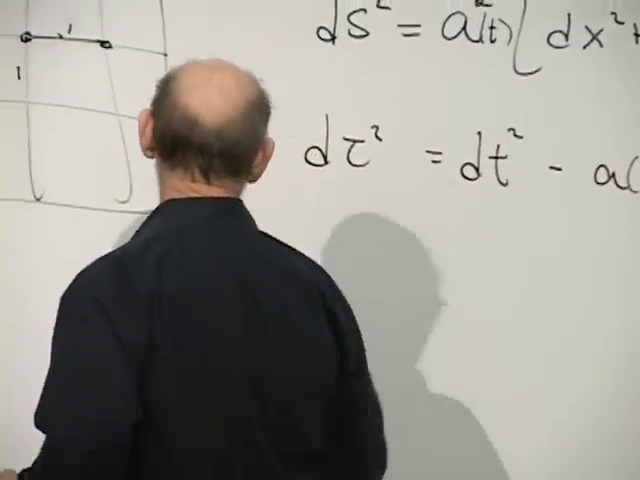
\includegraphics[width=0.62\textwidth]{lecture_02_figure_02.png}
\caption{Esquema de una retícula comóvil y del intervalo espacio-temporal con un factor de escala dependiente del tiempo.}
\end{figure}

La figura ilustra la idea. Alice y Bob permanecen separados por una unidad en las coordenadas comóviles, pero esa unidad de coordenadas representa cada vez más metros a medida que pasa el tiempo. Si \(a(t)\) hubiera sido cero en algún momento del pasado, todas las separaciones físicas habrían sido nulas: todo habría quedado aplastado junto. Por eso \(a\to 0\) corresponde a una densidad infinita. A medida que \(a\) crece, el universo se vuelve cada vez más difuso.

Esta forma de la métrica no es válida en todos los sistemas de referencia. Es la forma que tiene en el sistema que se mueve con las galaxias.

\begin{classroomqa}
\audiencequestion{En esa ecuación, la pequeña \(t\), \(a(t)\), ¿a qué tiempo \(t\) corresponde?}\lecturetimestamp{00:19:19}
\lecturerresponse{Es el tiempo que miden los relojes que se mueven con las galaxias. Imaginemos relojes idénticos, fabricados en la misma fábrica de relojes cósmicos y transportados por las galaxias. En este sistema de referencia, la variable temporal es exactamente lo que miden esos relojes. A lo largo de la línea de universo de una galaxia, el tiempo propio coincide con este tiempo coordenado.}
\end{classroomqa}

En efecto, a lo largo de la línea de universo de una galaxia comóvil,
\begin{equation}
dx=dy=dz=0,
\end{equation}
por lo que
\begin{equation}
d\tau^2 = dt^2,
\end{equation}
y, por tanto,
\begin{equation}
dt=d\tau.
\end{equation}

\begin{classroomqa}
\audiencequestion{¿Hay transformaciones que dejen invariante esta forma de la métrica?}\lecturetimestamp{00:23:08}
\lecturerresponse{Las rotaciones sí, porque \(dx^2+dy^2+dz^2\) es invariante bajo rotaciones. Las transformaciones de Lorentz, en cambio, no conservan esta forma. La propia materia selecciona el sistema de referencia que se mueve con las galaxias; en cualquier otro sistema, el universo no se vería isótropo.}
\end{classroomqa}

\section{Un proyectil en un campo gravitatorio}

Antes de aplicar las leyes de Newton al universo entero, conviene volver a un problema más sencillo: una masa grande \(M\), una masa mucho menor \(m\) y un impulso inicial hacia fuera. Después del impulso, la masa pequeña simplemente se mueve en el campo gravitatorio y hace lo que dictan las leyes de Newton.

Para la discusión cosmológica, lo importante no es resolver la órbita completa, sino la conservación de la energía. La energía cinética es
\begin{equation}
\frac{1}{2}mv^2.
\end{equation}

\begin{figure}
\centering
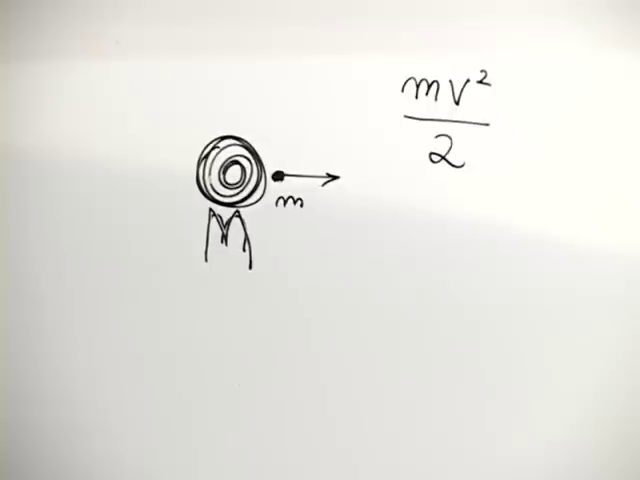
\includegraphics[width=0.42\textwidth]{lecture_02_figure_03.png}
\caption{Masa de prueba que se aleja y término de energía cinética \(\frac{1}{2}mv^2\).}
\end{figure}

La energía potencial gravitatoria contiene el producto de las masas, la constante de Newton y una potencia de la distancia en el denominador. En la expresión escrita en la pizarra, los factores aparecen en el orden \(mMG/D\), así que conviene conservar aquí ese orden:
\begin{equation}
-\frac{mMG}{D}.
\end{equation}
Por tanto, la energía total es
\begin{equation}
\frac{1}{2}mv^2-\frac{mMG}{D}.
\end{equation}
La conservación de la energía solo afirma que esta cantidad no cambia con el tiempo para la partícula en cuestión. Distintas partículas pueden tener energías distintas.

\begin{figure}
\centering
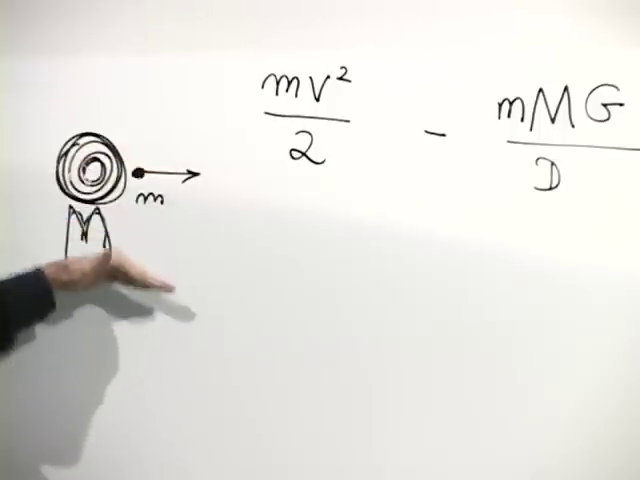
\includegraphics[width=0.62\textwidth]{lecture_02_figure_04.png}
\caption{Energía newtoniana total de una masa de prueba en movimiento radial: término cinético menos potencial gravitatorio.}
\end{figure}

El signo negativo es importante. La energía potencial gravitatoria es negativa porque la gravedad es atractiva. Al acercar la partícula, aumenta la magnitud de la energía potencial negativa. Al alejarla, la energía potencial se vuelve menos negativa.

\begin{classroomqa}
\audiencequestion{¿La energía potencial aumenta con la distancia en vez de disminuir?}\lecturetimestamp{00:34:13}
\lecturerresponse{Sí. Dejemos de lado las constantes y observemos las gráficas de \(1/D\) y \(-1/D\). La fuerza impulsa el movimiento hacia valores menores de energía potencial. Por tanto, una fuerza atractiva corresponde a la curva invertida, \(-1/D\): la energía potencial aumenta con la distancia y se hace más negativa a medida que la partícula se acerca.}
\end{classroomqa}

\begin{figure}
\centering
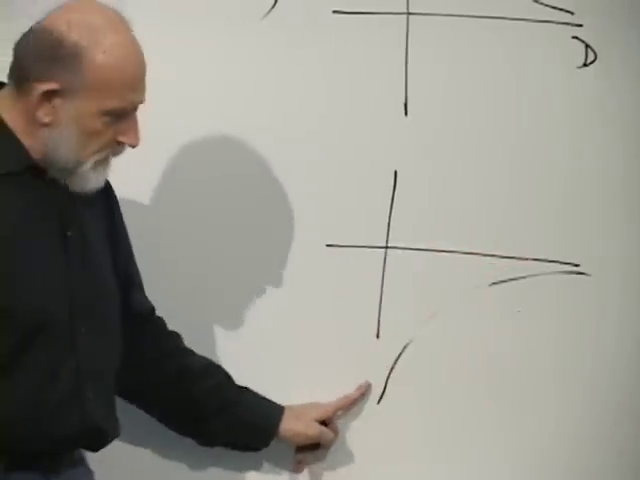
\includegraphics[width=0.46\textwidth]{lecture_02_figure_05.png}
\caption{Comparación cualitativa de \(1/D\) y \(-1/D\) para determinar el signo de la energía potencial gravitatoria.}
\end{figure}

\section{Velocidad de escape}

Clasifiquemos ahora las posibilidades. La energía puede ser positiva, negativa o nula. Esos son los únicos tres casos.

\begin{itemize}
\item Si la energía es negativa, la partícula está ligada. Si se la lanza hacia arriba con una velocidad demasiado pequeña, asciende, pierde velocidad, se detiene y vuelve a caer.
\item Si la energía es positiva, la partícula escapa. Al principio, la gravedad la desacelera, pero no lo suficiente como para detenerla, y al final se aleja con una velocidad de salida asintótica distinta de cero.
\item Si la energía es exactamente nula, la partícula tiene la velocidad de escape. Es el caso límite entre escapar y no hacerlo.
\end{itemize}

Si la velocidad inicial es suficientemente pequeña, el término potencial domina desde el principio y la energía es negativa.

\begin{figure}
\centering
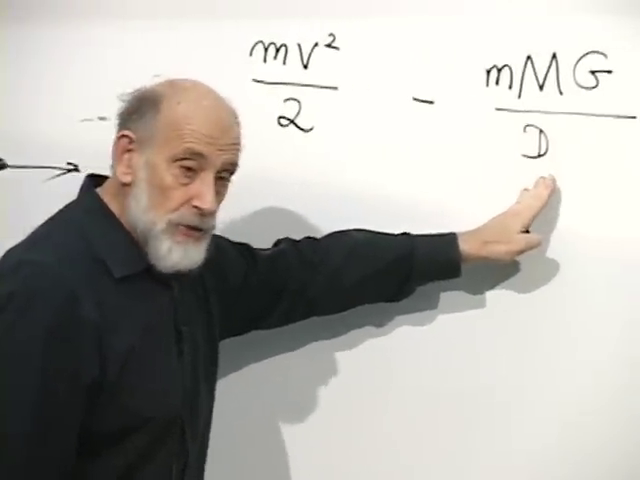
\includegraphics[width=0.62\textwidth]{lecture_02_figure_06.png}
\caption{A baja velocidad inicial hacia fuera, el término potencial negativo domina la energía total.}
\end{figure}

En el caso de energía nula, la distancia sigue aumentando, pero la rapidez sigue disminuyendo. La partícula no puede detenerse en ningún tiempo finito. Si lo hiciera, volvería a caer. Así pues, la distancia no está acotada, mientras que la velocidad tiende a cero.

Esta es la analogía directa que importa para la cosmología. El universo puede comportarse de la misma manera. Si el flujo de Hubble inicial hacia fuera es suficientemente grande, todo escapa de todo lo demás. Si es demasiado pequeño, la gravedad prevalece y se produce un gran colapso. También existe el caso límite, exactamente análogo a la velocidad de escape.

\section{Teorema de Newton}

La reducción cosmológica funciona gracias al teorema de Newton para la ley del inverso del cuadrado.

Si la materia está distribuida con simetría esférica alrededor de un centro, la fuerza gravitatoria sobre una partícula exterior a la distribución es exactamente la misma que si toda la masa estuviera concentrada en el centro. Pero el teorema es aún más potente. Si la partícula está dentro de la distribución, solo contribuye la masa situada a radios menores. La masa situada a radios mayores no produce fuerza neta.

La versión más clara del teorema es la de una cáscara esférica delgada. Una cáscara esférica perfecta no ejerce fuerza gravitatoria sobre ninguna partícula situada en su interior, ni siquiera si está fuera del centro. A primera vista sorprende, pero es cierto para la ley \(1/r^2\).

\begin{classroomqa}
\audiencequestion{En el ejemplo que acaba de dar, ¿no debería sorprendernos un poco que la fuerza parezca discontinua cuando la partícula cruza el límite?}\lecturetimestamp{00:48:19}
\lecturerresponse{Sí. Resulta sorprendente en el caso de una cáscara ideal infinitamente delgada, y es una propiedad exclusiva de la ley de fuerza \(1/r^2\). Una cáscara real tiene grosor, así que la variación se suaviza; pero la afirmación tajante para una cáscara ideal es precisamente la notable propiedad del teorema de Newton.}
\end{classroomqa}

Una imagen ayuda a hacer plausible el teorema. Sustituyamos una masa puntual por una fuente puntual de agua. En tres dimensiones, el flujo hacia fuera disminuye como \(1/r^2\). Dispongamos fuentes de ese tipo de manera continua por toda una cáscara esférica. Fuera de la cáscara, el flujo es exactamente igual que si todo estuviera concentrado en el centro. Dentro de ella no puede haber flujo neto, porque no hay ninguna fuente en el centro. Esa misma estructura es la que sustenta el teorema gravitatorio.

La idea aquí no es volver a demostrar el teorema, sino utilizarlo.

\section{Un universo homogéneo como problema de dos cuerpos}

Volvamos ahora a la cosmología. Tomemos una pequeña región del universo llena de un gas uniforme de galaxias. Si se quiere, uno puede situarse en el centro. Es solo una comodidad. Cualquiera puede decir que está en el centro, y debe resultar la misma ecuación.

Elijamos una galaxia sobre el eje \(x\), en la coordenada comóvil \(x\). Como el universo es isótropo, da igual qué eje escojamos. Tracemos una esfera centrada en \(x=0\) que pase por esa galaxia. Según el teorema de Newton, la fuerza sobre la galaxia es exactamente la misma que si toda la masa dentro de la esfera estuviera concentrada en el centro; todo lo que queda fuera no contribuye.

La esfera se expande junto con las galaxias. Siempre contiene las mismas galaxias y, por tanto, la misma masa total, aunque su radio físico cambie con el tiempo.

Por tanto, el movimiento de esa galaxia obedece exactamente al mismo tipo de ecuación de la energía que el proyectil:
\begin{equation}
\frac{1}{2}mv^2-\frac{mMG}{D}=\text{constant}.
\end{equation}
Aquí, \(M\) representa ahora la masa dentro de la esfera en expansión, no la masa central del ejemplo introductorio. Luego se simplifica el álgebra multiplicando por \(2\) y dividiendo por \(m\). Como una constante dividida por \(m\) sigue siendo simplemente una constante, podemos escribir
\begin{equation}
v^2-\frac{2MG}{D}=\text{constant}.
\end{equation}
De nuevo, ``constante'' significa constante en el tiempo para esa galaxia concreta.

Relacionemos ahora esto con el factor de escala. La distancia física a la galaxia es
\begin{equation}
D=ax,
\end{equation}
porque \(x\) es una coordenada comóvil fija. Su velocidad es
\begin{equation}
v=\dot D=\dot a\,x.
\end{equation}

La masa dentro de la esfera es la densidad multiplicada por el volumen. Si \(\rho\) es la densidad de masa, entonces
\begin{equation}
M=\frac{4\pi}{3}\rho D^3=\frac{4\pi}{3}\rho a^3x^3.
\end{equation}
Al sustituirlo en la ecuación de la energía se obtiene
\begin{equation}
\dot a^2x^2-\frac{2G}{ax}\left(\frac{4\pi}{3}\rho a^3x^3\right)=\text{constant},
\end{equation}
o bien
\begin{equation}
\dot a^2x^2-\frac{8\pi G}{3}\rho a^2x^2=\text{constant}.
\end{equation}

Los dos términos del lado izquierdo son proporcionales a \(x^2\). Todo lo demás en ese lado es igual en todas partes. Por lo tanto, el lado derecho también debe ser proporcional a \(x^2\). Esto no contradice que lo llamemos constante. Significa que es constante con respecto al tiempo para cada \(x\) fijo, pero aun así puede escalar con \(x^2\) de una galaxia a otra. Tiene sentido: las galaxias más lejanas se mueven más rápido.

Dividamos, pues, por el factor común \(x^2\). La constante restante ya es independiente tanto del tiempo como del espacio. Escribámosla de la forma históricamente convencional \(-k\):
\begin{equation}
\dot a^2-\frac{8\pi G}{3}\rho a^2=-k.
\end{equation}
Después de dividir por \(a^2\),
\begin{equation}
\left(\frac{\dot a}{a}\right)^2=\frac{8\pi G}{3}\rho-\frac{k}{a^2}.
\end{equation}

Esta es la famosa ecuación de Friedmann-Robertson-Walker, aunque en la clase también se señala que, en realidad, es la ecuación de Friedmann. La convención de signos es histórica. Escribir \(-k\) no significa que \(k\) tenga que ser positivo. \(k\) puede ser positivo, negativo o nulo. En unidades en las que la velocidad de la luz es igual a \(1\), \(k\) es adimensional.

\section{Densidad y ecuación para un universo dominado por la materia}

La siguiente pregunta es inmediata: ¿qué es \(\rho\)? No es constante. A medida que el universo se expande, la densidad disminuye.

Para expresar esa dependencia, tomemos un cubo unidad en el espacio de coordenadas: una unidad por lado en \(x\), \(y\) y \(z\). Las mismas galaxias permanecen dentro de ese cubo en todo momento porque el cubo se expande junto con las coordenadas. Así que la masa dentro de ese cubo de coordenadas permanece fija.

\editorialnote{En varias etapas, la clase reutiliza el símbolo \(M\). Aquí se usa \(M_{\Box}\) únicamente para distinguir la masa contenida en un cubo unidad de coordenadas de la masa central y la masa encerrada en la esfera anteriores.}

La longitud física de cada lado del cubo es \(a\), así que su volumen físico es \(a^3\). Por tanto,
\begin{equation}
\rho=\frac{M_{\Box}}{a^3}.
\end{equation}
Este es el caso dominado por la materia: el lado derecho contiene únicamente la densidad de la materia ordinaria no relativista.

\begin{classroomqa}
\audiencequestion{Según esa ecuación, la constante de Hubble es función de \(\rho\). Así que no es constante.}\lecturetimestamp{01:19:21}
\lecturerresponse{Exactamente. La constante de Hubble no es constante. Depende de la densidad, y la densidad cambia con el tiempo. Incluso se bromea en la clase con que el examen final podría consistir en una sola pregunta: ¿Es constante la constante de Hubble?}
\end{classroomqa}

Al sustituir \(\rho=M_{\Box}/a^3\) en la ecuación de Friedmann se obtiene
\begin{equation}
\left(\frac{\dot a}{a}\right)^2=\frac{8\pi G M_{\Box}}{3a^3}-\frac{k}{a^2}.
\end{equation}

En este punto quedan claras las elecciones arbitrarias. Se necesitan la masa contenida en un cubo unidad de coordenadas y el valor de \(k\). Los tres signos posibles de \(k\) corresponden a los tres casos de energía del problema del proyectil.

\begin{itemize}
\item Si \(-k>0\), la energía supera efectivamente la velocidad de escape y el universo se expande para siempre.
\item Si \(-k<0\), la gravedad acaba prevaleciendo y el universo vuelve a colapsar.
\item Si \(k=0\), el universo está exactamente en el caso de la velocidad de escape.
\end{itemize}

\begin{classroomqa}
\audiencequestion{¿Es \(k=0\)? Entonces, ¿la velocidad relativa entre dos galaxias se aproxima a cero?}\lecturetimestamp{01:21:12}
\lecturerresponse{Sí. En el caso crítico, la velocidad se aproxima a cero, pero la distancia sigue sin estar acotada. Las galaxias siguen separándose, aunque cada vez más despacio. Si de hecho se detuvieran en algún tiempo finito, volverían a caer.}
\end{classroomqa}

\section{El caso crítico \(k=0\)}

Elijamos ahora el caso más sencillo, \(k=0\). Es el caso exacto de la velocidad de escape y resulta más sencillo únicamente porque las matemáticas son más simples. La ecuación queda
\begin{equation}
\left(\frac{\dot a}{a}\right)^2=\frac{8\pi G M_{\Box}}{3a^3}.
\end{equation}

El lado derecho siempre es positivo y nunca se anula. Por tanto, \(\dot a/a\) no puede pasar por cero. En este caso, el universo no puede invertir el sentido de su evolución. O bien siempre se está expandiendo, o bien siempre se está contrayendo. Tomemos la rama de expansión.

Probemos ahora con una ley potencial,
\begin{equation}
a(t)=ct^p.
\end{equation}
Entonces
\begin{equation}
\dot a = cp\,t^{p-1},
\end{equation}
y, por tanto,
\begin{equation}
\frac{\dot a}{a}=\frac{p}{t}.
\end{equation}
Al sustituir en la ecuación diferencial se obtiene
\begin{equation}
\frac{p^2}{t^2}=\frac{8\pi G M_{\Box}}{3c^3t^{3p}}.
\end{equation}
Para que coincidan las potencias de \(t\), debe cumplirse
\begin{equation}
3p=2.
\end{equation}
Así que
\begin{equation}
p=\frac{2}{3}.
\end{equation}
Entonces, las constantes deben satisfacer
\begin{equation}
\frac{4}{9}=\frac{8\pi G M_{\Box}}{3c^3},
\end{equation}
de donde
\begin{equation}
c^3=6\pi G M_{\Box}.
\end{equation}
Por tanto,
\begin{equation}
a(t)=\left(6\pi G M_{\Box}\right)^{1/3}t^{2/3}.
\end{equation}

Todavía puede haber un desplazamiento aditivo en el tiempo. Se absorbe sustituyendo \(t\) por \(t-t_0\). Una vez que se elige el origen temporal de modo que \(a=0\) en \(t=0\), esa constante restante desaparece.

Así pues, el universo se expande según la potencia dos tercios del tiempo,
\begin{equation}
a(t)\propto t^{2/3}.
\end{equation}
No se expande linealmente con el tiempo. El crecimiento lineal sería análogo a un movimiento sin aceleración. En este caso, la expansión se desacelera.

Si prolongamos la fórmula hacia atrás hasta \(t=0\), el factor de escala tiende a cero y la densidad diverge. Decir \(a=0\) es una afirmación extrema. No sabemos qué ocurre con la materia cuando alcanza densidades demasiado altas. Lo esencial es que, en una etapa temprana, todo estaba tan apretado que los átomos, los núcleos y los quarks se encontraban juntos en un estado extraordinariamente denso.

\section{La constante de Hubble y la edad del universo}

En el modelo crítico,
\begin{equation}
H(t)=\frac{\dot a}{a}=\frac{2}{3t}.
\end{equation}
Así que la constante de Hubble es aproximadamente el inverso de la edad del universo,
\begin{equation}
t=\frac{2}{3H}.
\end{equation}
Este es uno de los principales resultados del cálculo. Si se mide la constante de Hubble hoy, se obtiene una estimación de la edad del universo, al menos hasta el punto en que el modelo newtoniano deja de tener sentido.

La edad que se cita es de aproximadamente \(13\) a \(14\) mil millones de años. El texto también señala que \(k=0\) concuerda muy bien con las observaciones: con el nivel de precisión indicado, no se conoce ninguna desviación significativa de \(k=0\).

\begin{classroomqa}
\audiencequestion{Me confunde un poco qué son \(M\) y \(a\).}\lecturetimestamp{01:39:16}
\lecturerresponse{Ambas cantidades dependen de cómo se elija la retícula. Si se cambia la caja de referencia, cambia la cantidad de materia que contiene y también el valor numérico del factor de escala. La magnitud física es la densidad, \(M/a^3\), o, de manera equivalente, combinaciones como \(a/M^{1/3}\), que no dependen de cómo se elija la retícula. En la solución con \(k=0\), la constante desconocida que multiplica a \(t^{2/3}\) se cancela en \(\dot a/a\), de modo que la relación de edad \(t=2/3H\) no depende de la masa de la caja de referencia.}
\end{classroomqa}

La cancelación se ve de inmediato en la solución. Si
\begin{equation}
a(t)=Ct^{2/3},
\end{equation}
entonces
\begin{equation}
\dot a=\frac{2}{3}Ct^{-1/3},
\end{equation}
y, por tanto,
\begin{equation}
\frac{\dot a}{a}=\frac{2}{3t}.
\end{equation}
La constante \(C\) desaparece por completo.

\section{Por qué funciona la derivación newtoniana}

Hacia el final, la pregunta pasa a ser: ¿por qué debería concordar tan bien la derivación newtoniana con la relativista?

\begin{classroomqa}
\audiencequestion{Todo esto parece depender del supuesto de que el universo es abierto.}\lecturetimestamp{01:45:44}
\lecturerresponse{En esta etapa, la derivación es newtoniana, y la física newtoniana supone un espacio plano. La interpretación de \(k\) en términos de la geometría del espacio se deja para la siguiente clase. Allí, \(k=0\) corresponderá a un espacio plano, mientras que los otros signos estarán vinculados a una geometría espacial curva.}
\end{classroomqa}

\begin{classroomqa}
\audiencequestion{Hace mucho tiempo, ¿dependía la longitud de las reglas métricas de \(a\)?}\lecturetimestamp{01:47:53}
\lecturerresponse{Si nos remontamos lo bastante, la materia habría estado tan apretada que las reglas métricas separadas ni siquiera habrían existido como tales. Antes de eso, se habrían comprimido. La clase también recuerda que la relatividad no permite la existencia de cuerpos perfectamente rígidos: si un cuerpo fuera perfectamente rígido, un empujón en un extremo enviaría una señal al otro al instante, más rápido que la luz.}
\end{classroomqa}

\begin{classroomqa}
\audiencequestion{¿Por qué cree que coinciden las ecuaciones newtoniana y relativista?}\lecturetimestamp{01:49:03}
\lecturerresponse{Porque el tratamiento newtoniano se aplica únicamente a una región suficientemente pequeña. Mientras la región sea pequeña en comparación con el radio de curvatura del universo entero y las velocidades de Hubble locales en ella sean mucho menores que la velocidad de la luz, la mecánica newtoniana constituye una buena aproximación. La clase lo compara con estudiar el crecimiento de la hierba en la Tierra: se puede entender el proceso local sin tener en cuenta la curvatura del planeta entero.}
\end{classroomqa}

Esta es la lógica de la región local. La mecánica newtoniana supone, primero, que la curvatura del espacio no es relevante para la cuestión que se estudia y, segundo, que nada se mueve localmente a una velocidad cercana a la de la luz. En cosmología, eso significa elegir una región suficientemente grande para que sea homogénea, pero lo bastante pequeña para que los efectos de la curvatura sean despreciables y las velocidades de Hubble sigan siendo no relativistas.

Con esto en mente, el cálculo newtoniano no es una coincidencia. Es la aproximación local de una ecuación que también puede expresarse en forma relativista. Si se pasa el término de curvatura al lado izquierdo, la ecuación de Friedmann queda
\begin{equation}
\left(\frac{\dot a}{a}\right)^2+\frac{k}{a^2}=\frac{8\pi G}{3}\rho.
\end{equation}
El lado izquierdo es geométrico: contiene el factor de escala y, en la próxima clase, la curvatura del espacio. El lado derecho es la densidad de energía. Es exactamente el tipo de ecuación que se espera de la relatividad general.

La próxima vez estudiaremos la curvatura en sí, las ecuaciones de Einstein y la relación entre esa derivación relativista y la newtoniana.
